% -*- root: 00-main.tex -*-
\section{Methods}
\label{sec:methods}
%

\subsection{Susceptibility-derived distortions}
\label{sec:distortions}
\Gls*{dmri} data are usually acquired with \gls*{epi} schemes.
In order to quickly probe the diffusion process within the brain in many different orientations,
  these sequences minimize the bandwidth of the \gls*{pe} direction.
This low bandwidth originates the artifactual displacement of locations presenting small deviations
  from the main magnetic field $B_0$.
The principal source of these deviations ($\Delta B_0$) is the discontinuity of magnetic
  susceptibility at tissue interfaces.
Tissue/air boundaries show large steps of susceptibility and this artifact is
  particularly evident in the surroundings of the orbito-frontal lobe or the temporal
  bone of both hemispheres.
The displacements field $U_s$ along the \gls*{pe} axis can be estimated theoretically
  \citep{jezzard_correction_1995}:

  \begin{equation}
  \vec{r}' = \vec{r} + \frac{\gamma \, T_{acq}\, s_{PE}}{2\pi}\Delta B_0(\vec{r}) \cdot \hat{\vec{e}}_{PE},
  \label{eq:fieldmap}
  \end{equation}
%
where $\vec{r}$ is the true location in the undistorted domain as in \eqref{eq:transform},
  $\gamma$ is the gyromagnetic ratio, $T_{acq}$ is the readout time,
  $s_{PE}$ is the pixel spacing along \gls*{pe}, and $\hat{\vec{e}}_{PE}$ the unitary
  vector along \gls*{pe}.
Several methodologies have been proposed to estimate $U_s$ and fix the artifact.
The first solution consisted on estimating $\Delta B_0$ with field mapping
  techniques \citep{andersson_modeling_2001}.
A second family of methods require an extra \gls*{epi} acquisition, but switching
  the \gls*{pe} axis \citep{chiou_simple_2000} or reversing the direction of gradient \gls*{pe}
  increments \citep{cordes_geometric_2000,holland_efficient_2010}.
\cite{kybic_unwarping_2000} proposed a correction using nonlinear registration of the \emph{b0}
  image\footnote{The term \emph{b0} refers to one or more images within the
  \gls*{dmri} dataset that are acquired with a null or very low gradient intensity or
   \emph{b}-value used as signal reference.} of the \gls*{dmri} versus a \gls*{t2} image.
Further developments \citep{irfanoglu_susceptibility_2011} extended this method to the
  three-dimensional problem.
Therefore, a typical protocol for the extraction of structural connectivity
  comprehends \gls*{dmri}, \gls*{t1}, and the acquisition determined by the correction
  method of choice \citep{daducci_connectome_2012}.


\subsection{Our method and contributions}
\label{sec:our_method}
\emph{Regseg} is related to \emph{bbregister}, as both methods exploit the precise
  surfaces that can be extracted with \emph{FreeSurfer}~\citep{fischl_freesurfer_2012},
  to then map this prior information into a target image.
However, \emph{bbregister} features an affine transform that is unable to compensate the
  distortions.
To avoid this problem, the active contours are dismissed in regions typically affected by
  warpings.
Additionally, \emph{bbregister} is robust in finding clear tissue boundaries.
In the case of \gls*{dmri} data, oftentimes the registration process is restricted to finding
  the pial surface, as it is the only clear boundary.

to the methods based on nonlinear registration of the
  to the \gls*{t2} image, since we also render the correction as a
  registration problem.
Conversely, the method does not require any of the previously mentioned extra acquisitions.
A fundamental antecedent to \emph{regseg} is found in .
They proposed a registration method to align surfaces extracted from the \gls*{t1}
  to \gls*{dmri} images using a linear transformation model using active contours
  with edges.
Similarly, we  warped data, in which the scale of the
  imaged structures is in the range of the image resolution or above.
Our approach differs from \citep{greve_accurate_2009} in two fundamental choices.
First, we use a nonlinear deformation model that enables the correction of the
  susceptibility-derived distortions \citep{jezzard_correction_1995}.
\cite{greve_accurate_2009} circumvented the nonlinearity by identifying typically
  distorted regions and removing them from the metric computation.
Second, our matching criteria does not necessarily need for clear intensity
  steps at the tissue interfaces where surfaces must be fitted, thanks to the use of
  active contours without edges \citep{chan_active_2001}.


This choice is similar to \citep{guyader_combined_2011}, but \emph{regseg} differs in two
  features.
First, the regularization relies on the inherent smoothness of the deformation field,
  and on the anisotropic approach proposed by \cite{nagel_investigation_1986}.
Second, it accepts several contours to be mapped as in \citep{gorthi_active_2011}.
However, \emph{regseg} makes use of the explicit representation of surfaces, and
  does not implement multiphase level sets.
Our registration method is demonstrated here as a solution to correct for the susceptibility
  distortions that \gls*{dmri} of the head typically present \citep{jezzard_correction_1995}.
The distortion correction and the precise segmentation of \gls*{dmri} data is crucial in
	applications such as connectome extraction \citep{craddock_imaging_2013}, since the
  definition of the nodes in the network is generally derived from a parcellation performed in
  an anatomical \gls*{mri} of the same subject \citep{daducci_connectome_2012}.



\subsection{Cost-function derivation}\label{sec:methods_map}

In a Bayesian framework, the mappings $U$ in \eqref{eq:transform} are
  evaluated based on their posterior probability given the observed data
  $R$.
Using the Bayes' rule, the posterior likelihood is computed as:

  \begin{equation}
  P(U \mid R,\Gamma_{l,m}) = \frac{P(R \mid U,\Gamma_{l,m})\, P(U)}{P(R)},
  \label{eq:bayes_rule}
  \end{equation}

  where $P(R \mid U,\Gamma_{l,m})$ is the data-likelihood, and
  $\Gamma_{l,m}$ are a set of surfaces corresponding to the interfaces
  between piecewise smooth regions $\Omega_i$, such that
  $\Gamma_{l,m} = \partial \Omega_l \cap \partial \Omega_m$ is the
  contour between competing regions $\Omega_l$ and $\Omega_m$.
The best estimate $\hat{U}$ then fulfills the maximum a posteriori criterium
  \citep{bishop_pattern_2006}, and aligns $\Gamma$ into $R$.

First, we assume independence between pixels, and thus break down the
  global data likelihood into a product of pixel-wise conditional probabilities:

  \begin{equation}
  P(R \mid U,\Omega) = \underset{l}{\prod} \underset{\vec{r}\in \Omega_l}{\prod}
    P\left( \vec{f}' \mid U \right),
  \label{eq:bayes_aposteriori}
  \end{equation}

  where $\vec{f}' = R(\vec{r}')$ is the feature vector at the displaced
  position $\vec{r}'$ \eqref{eq:transform} in the multispectral target
  volume.
For convenience, and because it has been shown to be an appropriate approximation
  \citep{leemput_automated_1999,cuadra_comparison_2005}, we introduce two assumptions for each
  region $\Omega_l$:
  1) the features are i.i.d.; and 2) they can be modeled by multivariate normal
  distributions with parameters $\lbrace \boldsymbol{\mu}_l, \boldsymbol{\Sigma}_{l} \rbrace$
  for each region $\Omega_l$.
We then insert the normal distribution into \eqref{eq:bayes_rule} to obtain the full
  formulation of the \emph{data term} of our registration model:

 	\begin{align}
  P( R \mid U, \Omega ) &= \underset{l}{\prod} \underset{\vec{r} \in \Omega_l}{\prod}
  \mathcal{N} ( \vec{f} \mid \boldsymbol{\mu}_l, \boldsymbol{\Sigma}_{l} ) \notag\\
  &= \underset{l}{\prod} \underset{\vec{r} \in \Omega_l}{\prod} \frac{1}{ \sqrt{(2\pi)^{C}\,\left|\boldsymbol{\Sigma}_{l}\right|}}\,{e^{\left(-\frac{1}{2}
  \mdist{f'}{l} \right)}},
  \label{eq:pdf}
  \end{align}

  using $\mdist{f}{l}$ to denote the squared \emph{Mahalanobis distance} of $\vec{f}$ with respect
  to the descriptors of region $l$ as
  $\mdist{f}{l} = (\vec{f} - \boldsymbol{\mu}_l)^T \, {\boldsymbol{\Sigma}_l}^{-1} \, (\vec{f} - \boldsymbol{\mu}_l)$.


The smoothness of the resulting displacements field is induced by a Thikonov regularization
  prior:

  \begin{align*}
  P(U) = \underset{\vec{r}}{\prod}\, p(u(\vec{r})) &=
  \underset{\vec{r}}{\prod}\, p_0(u(\vec{r})) \, p_1(u(\vec{r})), \\
  p_0(u(\vec{r})) &= \mathcal{N}( u(\vec{r}) \mid 0, \mathbf{A}^{-1}), \notag\\
  p_1(u(\vec{r})) &= \mathcal{N}(  \nabla \cdot u(\vec{r}) \mid 0, \mathbf{B}^{-1}),
  \end{align*}

  imposing that the distortion and its gradient have zero
  mean and variance governed by the matrices $\mathbf{A}$ and $\mathbf{B}$.
Since the anisotropy is generally aligned with the imaging axes, these will be simplified
  in the following for the sake of clarity:

  \begin{align}
    p_0(u(\vec{r})) &= \underset{\vec{r}}{\sum} \mathcal{N}( u(\vec{r}) \mid 0,
      (\boldsymbol{\alpha}^{\circ\frac12}\,\vec{I}_n)^{-1}), \notag\\
    p_1(u(\vec{r})) &= \underset{\vec{r}}{\sum} \mathcal{N}( \nabla \cdot u(\vec{r}) \mid 0,
      (\boldsymbol{\beta}^{\circ\frac12}\,\vec{I}_n)^{-1}).
  \label{eq:priors}
  \end{align}


Finally, the maximum a posteriori problem is adapted into a variational one where we look for
  the minimum of an energy functional, by applying a log-transform:

  \begin{align}
  E(R \mid U) &= -\log \underset{l}{\prod}
  \underset{\vec{r} \in \Omega_l}{\prod}
  \mathcal{N} \left( \vec{f}' \mid \Theta_l \right)\,p_0( u(\vec{r}))\,p_1( u(\vec{r})) \notag\\
  &= C + \underset{l}{\sum} \int_{\Omega_l}
  \mdist{f'}{l} \,d\vec{r} \notag\\
  &+ \int_{\Omega} \left[ \boldsymbol{\alpha} \cdot u(\vec{r})^{\circ2}
  + \boldsymbol{\beta} \cdot (\nabla \cdot u(\vec{r}))^{\circ2} \right] \,d\vec{r},
  \label{eq:energy}
  \end{align}

  this expression is dual to the energy functional corresponding
  to a discrete \gls*{acwe} framework \citep{chan_active_2001}
  with the corresponding anisotropic regularization term \citep{nagel_investigation_1986}.


\subsection{Numerical Implementation}
\label{sec:numerical_implementation}

\begin{figure}
	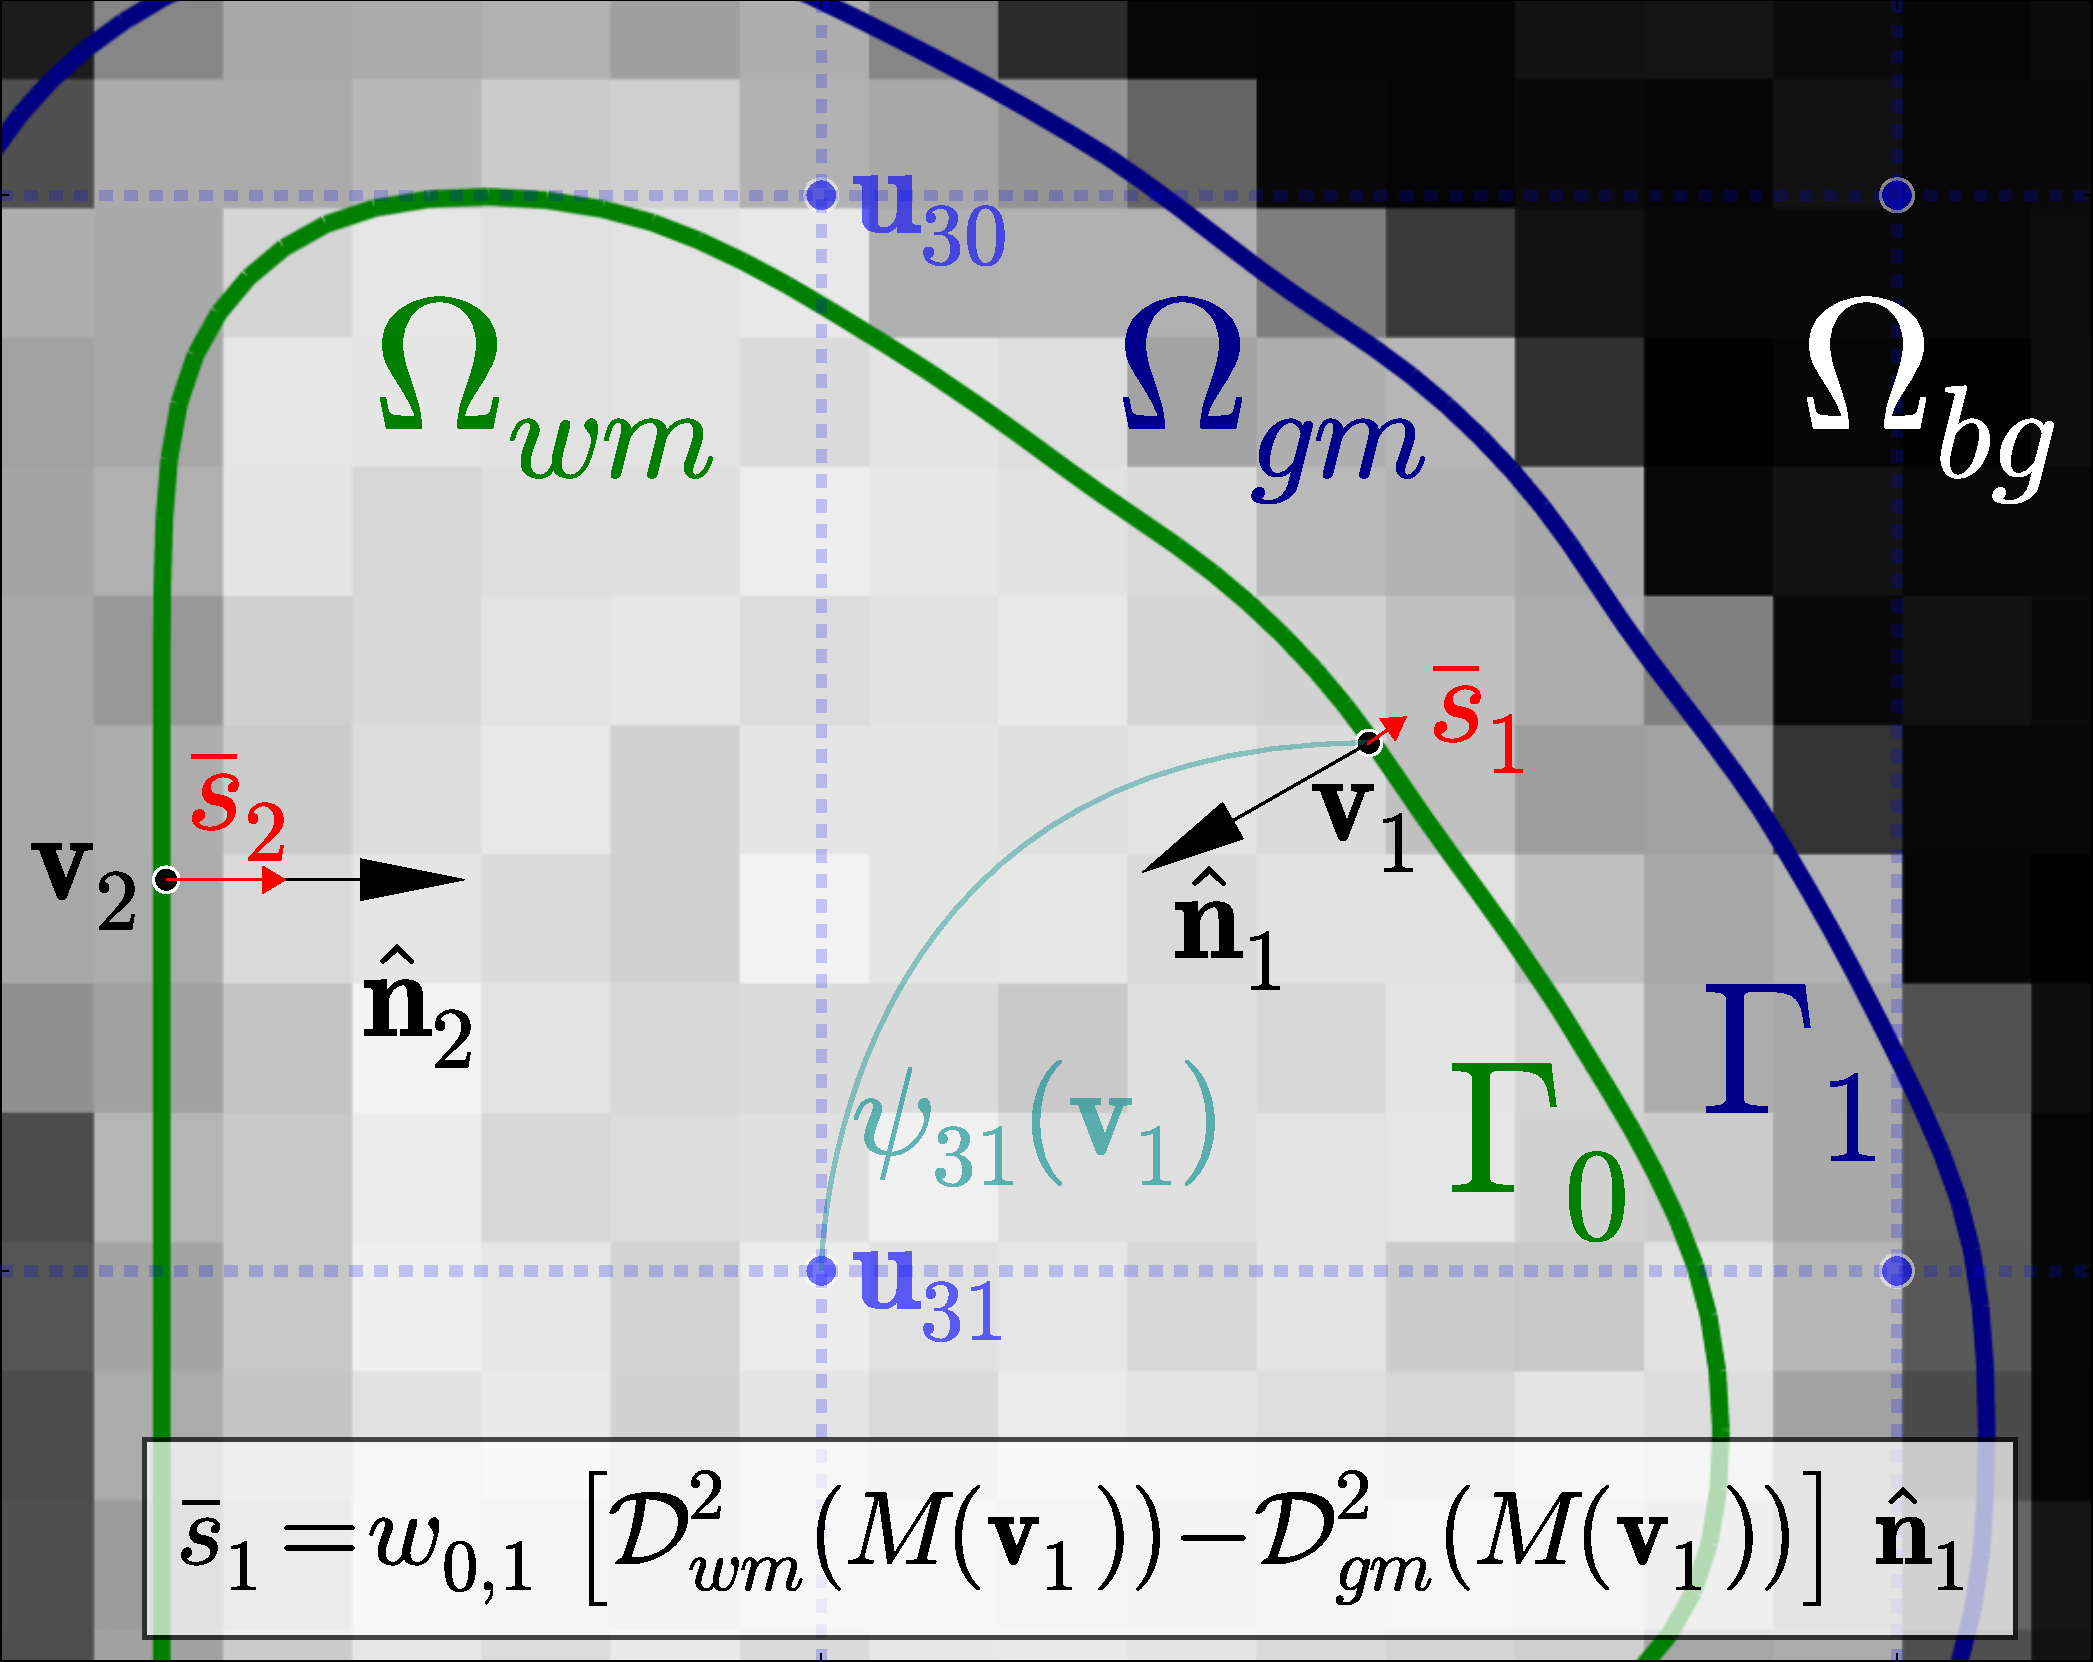
\includegraphics[width=\linewidth]{figures/figure01}
	\caption{The active contours are defined as the interfacing surfaces of the competing
	  \glspl{roi} $\Omega_i$.
	They are represented in green and dark blue colors in this close-up.
	They iteratively evolve following their inner normals $\hat{n}_i$ at each vertex
	  $\vec{v}_i$ of the mesh.
	The gradient speeds $\bar{s}_i$ are computed as the disparity between data energies of
	  the vertex $\vec{v}_i$ in each limiting region (see \autoref{app:shape_priors}).
	In this figure, the gradient speed corresponding to $\vec{v}_1$ is written in the lower
	  box, $\Omega_{wm}$ being the inner limiting region and $\Omega_{gm}$ the outer.
	Finally, every $\bar{s}_i$ is associated with the control points $\vec{u}_k$ through
	  the corresponding weights $\psi_k(\vec{v}_i)$ \eqref{eq:basis_derivative}.
	}\label{fig:method}
\end{figure}

\paragraph*{Deformation model}\label{sec:deformation_model}
Let us denote $\{\vec{v}_i\}_{i=1 \ldots N_c}$ the vertices of one or several prior
  surface(s).
In our application, these surfaces are triangularized meshes extracted using \emph{FreeSurfer}
  \citep{fischl_freesurfer_2012}.
The transform $\hat{U}$ \eqref{eq:transform} is supported by a dense deformation field
  $u(\vec{r})$, such that:

  \begin{equation}
  \vec{v}_i' = \hat{U}\{\vec{v}_i\} = \vec{v}_i + u(\vec{v}_i).
  \label{eq:nodes_tfm}
  \end{equation}

Since the nodes of the anatomical surfaces likely lay off-grid, it is required to
  derive $u(\vec{r})$ from a discrete set of parameters $\{\vec{u}_k\}_{k=1 \ldots K}$.
Densification is achieved through a set of associated basis functions $\psi_k$:

  \begin{equation}
  u(\vec{r}) = \sum_k \psi_k(\vec{r}) \vec{u}_k.
  \label{eq:intp_kernel}
  \end{equation}

In our implementation, $\psi_k$ is chosen to be a tensor-product B-Spline kernel
  of degree 3 ($\beta_3$).
Then, introducing \eqref{eq:intp_kernel} into \eqref{eq:nodes_tfm} and replacing
  $\psi$ by the actual kernel function, the transformation writes:

  \begin{equation}
    \vec{v}_i' = \vec{v}_i + \sum_k \left[ \vec{u}_k \, \underset{d}{\prod}
      \beta_3( (\vec{v}_i - \vec{r}_k) \cdot \hat{\mathbf{e}}_d ) \right],
  \label{eq:transformation}
  \end{equation}

  with $\hat{\mathbf{e}}_d$ being the unitary vector along axis $d$.


\paragraph*{Optimization}
\label{sec:gradient_descent}
To find the minimum of the energy functional \eqref{eq:energy},
  we propose a gradient-descent approach with respect to the underlying
  deformation field through the following \gls*{pde}:

  \begin{equation}
  \frac{\partial u(\vec{r},t)}{\partial t} \propto - \frac{\partial E(\vec{u})}{\partial \vec{u}_k},
  \label{eq:general_gradient_descent}
  \end{equation}

  with $t$ being an artificial time parameter of the contour
  evolution, and $\vec{u}_k$ the parameters supporting the estimate
  $\hat{U}$ of the transformation at the current time point.
Now, we introduce \eqref{eq:energy} in \eqref{eq:general_gradient_descent}:

  \begin{align}
  \frac{\partial E(\vec{u})}{\partial \vec{u}_k} &=
  \frac{ \partial }{\partial \vec{u}_k} \Big\{
  \int_{\Omega} \underset{l}{\sum} \mdist{f'}{l} \,d\vec{r} \notag\\
  &+ \int_{\Omega} [ \boldsymbol{\alpha} \cdot u(\vec{r})^{\circ2}
  + \boldsymbol{\beta} \cdot (\nabla \cdot u(\vec{r}))^{\circ2} ] \,d\vec{r}
  \Big\}.
  \label{eq:gradient_descent}
  \end{align}


We can apply a discretized interpretation of \eqref{eq:shape_gradients} to compute
  the data term in \eqref{eq:gradient_descent} using shape-gradients
  \citep{herbulot_segmentation_2006}, and ultimately avoid level sets.
We refer the reader to the appendix \autoref{app:shape_priors} in order to fill in the gap
  between \eqref{eq:gradient_descent} and the following expression:

  \begin{align}
  \frac{\partial E_{data}(\vec{u})}{\partial \vec{u}_k} &=
  \frac{ \partial }{\partial \vec{u}_k} \left\{
   \underset{\vec{x} \in \Omega_l}{\sum} \underset{l}{\sum} \mdist{f'}{l} \right\}
  = \underset{i}{\sum}
   \left\langle \frac{\partial \vec{v}_i'}{\partial \vec{u}_k}, \bar{s}_i'\right\rangle,
  \label{eq:gradient_wshape}
  \end{align}

  in this case, the formulation has been adapted to the non-binary case, $\{l,m\}$
    being any pair of neighboring regions, and $\Gamma_{l,m}$ the contour separating
    them such that
    $\vec{x}' = \vec{v}' \in\Gamma_{l,m} \iff \vec{x}\in \partial\Omega_i \cap \partial\Omega_j$
    and $\bar{s}_i'$ is the speed vector projected on to the unit inward normal to the contour
    at $c_i'$ (described in \autoref{fig:method}).


Finally, we can compute:

  \begin{align}
  \frac{\partial \vec{v}_i'}{\partial \vec{u}_k} &= \frac{\partial}{\partial \vec{u}_k}
  \left\{ \vec{v}_i + \sum_k \psi_k(\vec{v}_i) \vec{u}_k \right\}
  = \psi_k(\vec{v}_i)\, \hat{\vec{e}}
  \label{eq:basis_derivative}
  \end{align}

  where $\hat{\vec{e}}$ is the coordinates system's unit vector.
The vertex speeds $\bar{s}_i'$ obtained by computing the shape-gradients \eqref{eq:shape_gradients},
	are then projected to the deformation field in order to obtain the derivatives $\vec{g}_k$
	corresponding to $\vec{u}_k$:

  \begin{equation}
  \vec{g}_{i,k} = \left\langle \frac{\partial}{\partial \vec{u}_k}{\vec{v}_i}', \bar{s}_i'\right\rangle
  = - \left[ \mdist{f_i'}{l} - \mdist{f_i'}{m} \right] \psi_k(\vec{v}_i)\, \hat{\vec{e}},
  \end{equation}

  then the full gradient evolution equation \eqref{eq:gradient_descent} yields:

  \begin{align}
  \frac{\partial E(\vec{u}_k)}{\partial \vec{u}_k} =
  &\underset{i}{\sum} \vec{g}_{i,k} +2\, \boldsymbol{\alpha} \vec{u}_k
  -2\, \boldsymbol{\beta} \Delta \vec{u}_k,
  \label{eq:gradient_final}
  \end{align}

\todo[inline]{Include here the final update equation using the FT, introducing the
step size $\tau$, and refer to the supplementals for intermediate steps}

\paragraph*{Settings, implementation details, and convergence}
\label{sec:conv_report}
The registration parameters (such as $\tau$, the B-Spline grid resolutions,
  target image smoothing, etc.) and implementation details (for instance the sparse matrix approach
  to fast interpolation) are discussed in the \suppl{}, section S1.
The actual choices of parameter settings are publicly distributed with the source code of the experiments.
Additionally, we release our software along with a tool for generating convergence reports to
  demonstrate the behavior of \emph{regseg} and help scientists configure their own experiments.
One sample report is found in the \suppl{}, section S1.3.


\subsection{Experiments and evaluation}
\label{sec:experiments_evaluation}
%
In order to demonstrate the performance of \emph{regseg}, we first conducted a battery of
  accuarcy tests over synthetic data, and then applied it in the susceptibility distortion
  correction of real data.
\autoref{fig:evworkflows} presents the workflow implementing the evaluation instruments.
Besides a visual assessment of the results, we report quantitative evaluations using
  two metrics.
In the case of the phantoms, since we had produced distortions along the three
  available dimensions, we computed the Haussdorf distance, by reusing the
  ``point-to-cell'' method of \cite{commandeur_vtk_2011}.
Conversely, the susceptibility-derived distortions only happen along the \gls*{pe}
  axis of the image.
Therefore, a \gls*{swindex} can be computed as the one-to-one distance between corresponding
  vertices of surfaces, weighted by their respective Voronoi area $w_i$:

  \begin{equation}
  sWI = \frac{1}{P} \sum\limits_p^P \frac{1}{A_p} \sum\limits_i^{N_p} w_i\,\|
  \vec{v}_i - \hat{\vec{v}}_i \|
  \label{eq:swindex}
  \end{equation}

  where $\vec{v}_i$ are the locations of the $N_p$ vertices in each $p \in \{1, \dots P\}$
  prior, $A_p$ the total area of surface $p$, and $\hat{\vec{v}}_i$ is the location
  recovered corresponding to the vertex $\vec{v}_i$.


\begin{figure*}
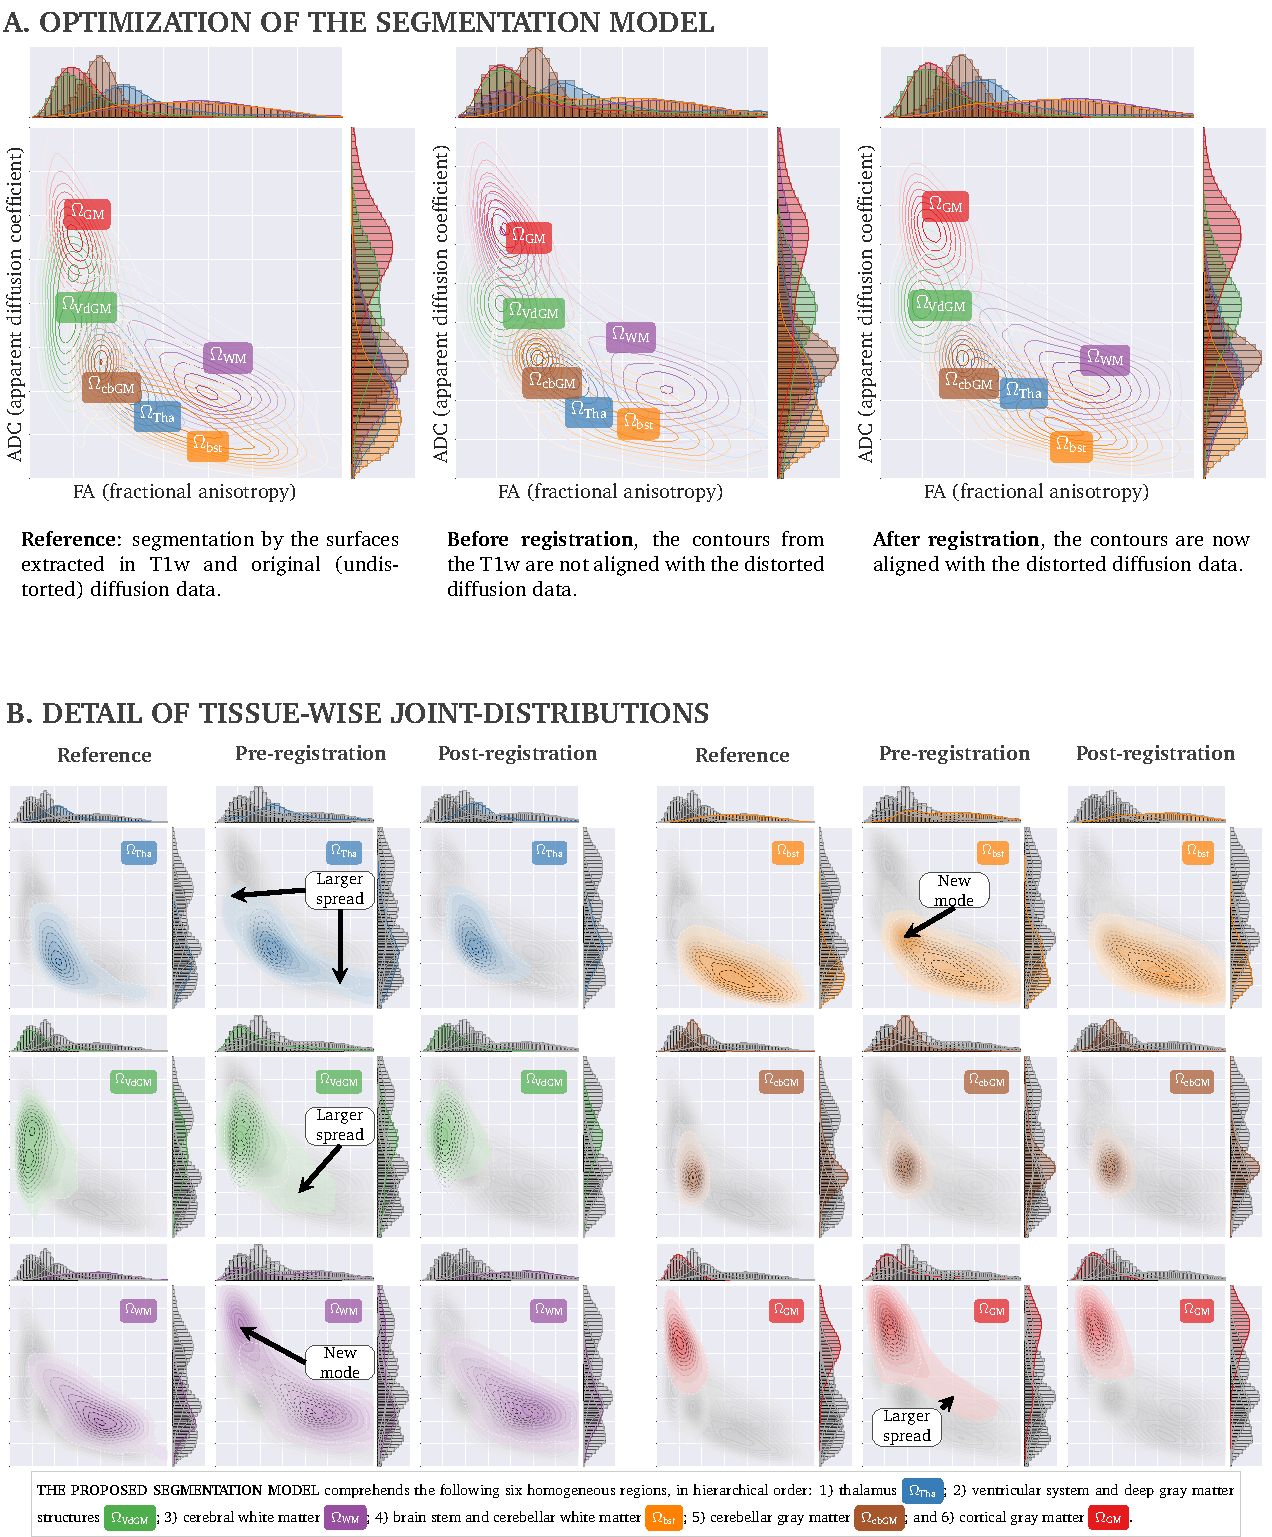
\includegraphics[width=\linewidth]{figures/figure02}
\caption{Experimental workflow applied on real data from the \acrfull*{hcp}.
  1) The prior surfaces are extracted from the anatomical reference (\gls*{t1} image).
	2) To operate as ground truth, we generate a plausible-synthetic distortion $U_{true}$
	  from the fieldmap using \eqref{eq:fieldmap}.
	3) The \gls*{dmri} data are warped using $U^{-1}_{true}$ to reproduce the effects of real
	  susceptibility-derived distortions.
	Target diffusion scalars (\gls*{fa} and \gls*{adc}) are computed on the distorted data and
		stacked to feed the multivariate input required by our algorithm.
	4) \emph{Regseg} is run, obtaining a $U_{test} = \hat{U}_{true}$, the estimation of
	  the ground-truth deformation.
	  A cross-comparison methodology is also applied, to obtain a competing $\hat{U}_{cc}$.
	5) Results are visually and quantitatively evaluated.}\label{fig:evworkflows}
\end{figure*}


\subsection{Image Data and preprocessing}
\label{sec:datasets}

\paragraph*{Simulated phantoms}%
\label{sec:digital_phantoms}
We proved the concept on simplistic digital phantoms which we will name after their
  appearance as ``box'', ``ball'', ``L-shape'', and ``gyrus'' (\autoref{fig:phantom},
  boxes A and B).
Using \emph{phantomas} \citep{caruyer_phantomas_2014}, we simulated
  \gls*{t1} (TE/TR=10/1500ms) and \gls*{t2} images (TE/TR=90/5000ms)
  corresponding to each phantom type, with two resolutions each
  ($1.0mm$ and $2.0mm$ isotropic).
Simulations were corrupted with rician noise for a \gls*{snr} of 300.0.
The reference surfaces were extracted using the marching-cubes algorithm
  shipped with \emph{FreeSurfer} \citep{fischl_freesurfer_2012}
  at the higher resolution (1.0mm isotropic).

\begin{figure*}
	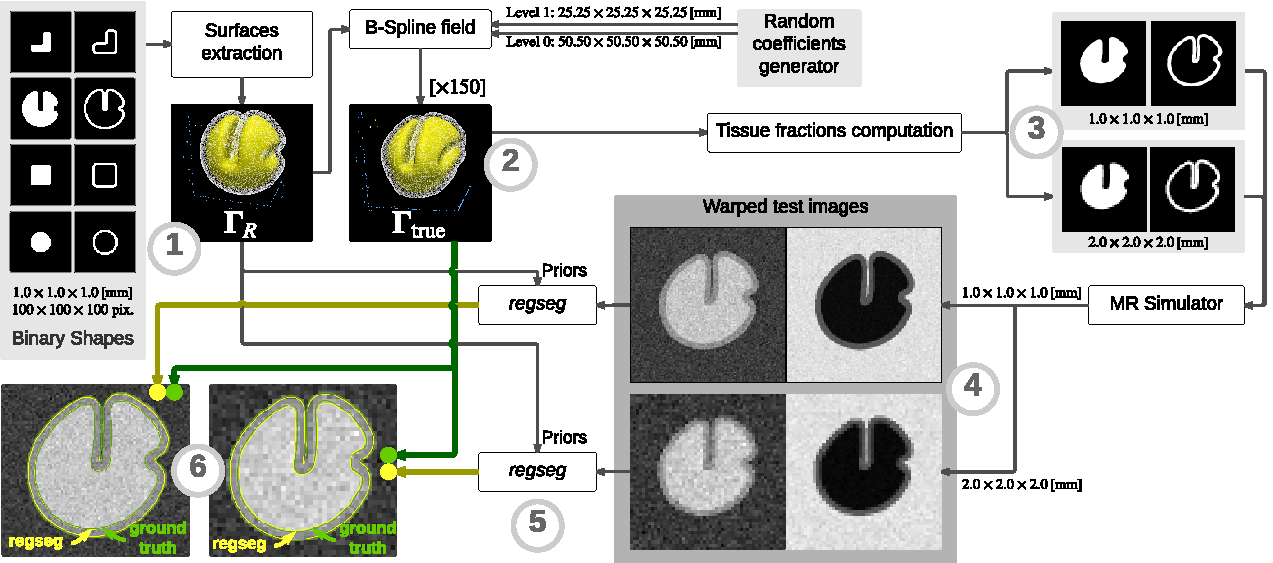
\includegraphics[width=\linewidth]{figures/figure03}
	\caption{A. The ``cortex'' phantom is a spherical shape with two sulci and an
	  outer crust resembling the cortical folding (left).
	The model is used to generate \gls*{t1} and \gls*{t2} images after warping the
	  contours using a random and plausible transformation $U_{true}^{-1}$ (right).
	B. Visual assessment of the results on the low resolution sets:
	  ``gyrus'' (top-left), ``L-shape'' (top-right), ``ball'' (bottom-left),
	  and ``box'' at (bottom-right).
	In yellow color, the recovered contours after registration are represented.
	Our method showed high accuracy, as they are overlapping the ground truth surfaces
	  depicted in green.
	Partial volume effect turns segmentation of the sulci a challenging problem with voxel-wise
	  clustering methods, but it is successfully segmented with our method.
	C. Quantitative evaluation of registration error in terms of average Hausdorff distance of
	  surfaces at high (left) and low (right) resolutions, demonstrating that the error is
	  consistently below the image resolution.
	  }\label{fig:phantom}
\end{figure*}

\paragraph*{Real datasets} %
\label{sec:human_connectome}
%
For the evaluation of the algorithm on real \gls*{dmri} data of human brains,
  we collected 16 datasets from the ``minimally preprocessed''
	 database of the \gls*{hcp}.
\todo[inline]{This is partially true: I am currently processing the data and
only 5 subjects with regseg and 10 with the competing method are processed.
All the results presented afterwards are based on this processed cases, and will be
updated for the final submission.}
We refer the reader to \citep{essen_human_2012} for exact details about acquisition
  parameters, and \citep{glasser_minimal_2013} for the preprocessing issues.
The datasets comprehend a large set of images, containing \gls*{t1}, \gls*{t2} and
  multi-shell \gls*{dmri} images.
The original acquisitions are released within ``unprocessed'' packages, and
  the ``minimally preprocessed'' are corrected for artifacts, brain-extracted
  and spatially normalized, along with some results of the standard processing
  pipeline of \emph{FreeSurfer}.

Selecting the appropriate labels in the \emph{aparc} segmentation, we applied
  the marching-cubes algorithm again to extract the surface of the following
  six homogeneous regions $\Omega_l$:
  1) the thalamus, $\Gamma_{Tha}$;
  2) \gls*{csf} of the ventricular system and deep \gls*{gm} structures, $\Gamma_{VdGM}$;
  3) cerebral \gls*{wm}, $\Gamma_{WM}$;
  4) brain stem and cerebellar \gls*{wm}, $\Gamma_{Bst}$;
	5) cerebellar \gls*{gm}, $\Gamma_{cbGM}$; and
	6) cortical \gls*{gm} surface, $\Gamma_{pial}$.
The choice of this particular model is further addressed in \autoref{sec:res_model_and_metric}.

In this case, we derived the deformation $U_{true}$ from the field maps released with
  the corresponding packages of each dataset from the \gls*{hcp} applying \eqref{eq:fieldmap},
  mimicking the real distortions, using a derivation of our previous work
  \citep{esteban_simulationbased_2014}.
After warping the original \gls*{dmri} with $U_{true}^{-1}$, we computed the \gls*{dti} and
  the derived scalars (\gls*{fa} and \gls*{adc}) using \emph{MRtrix} \citep{tournier_mrtrix_2012}.